\documentclass{article}

% if you need to pass options to natbib, use, e.g.:
%     \PassOptionsToPackage{numbers, compress}{natbib}
% before loading neurips_2021
\PassOptionsToPackage{square, numbers}{natbib}
% ready for submission
\usepackage{neurips_2021}
\usepackage{multirow}
\usepackage{float}
% to compile a preprint version, e.g., for submission to arXiv, add add the
% [preprint] option:
%     \usepackage[preprint]{neurips_2021}

% to compile a camera-ready version, add the [final] option, e.g.:
%     \usepackage[final]{neurips_2021}

% to avoid loading the natbib package, add option nonatbib:
%    \usepackage[nonatbib]{neurips_2021}

\usepackage[utf8]{inputenc} % allow utf-8 input
\usepackage[T1]{fontenc}    % use 8-bit T1 fonts
\usepackage{hyperref}       % hyperlinks
\usepackage{url}            % simple URL typesetting
\usepackage{booktabs}       % professional-quality tables
\usepackage{amsfonts}       % blackboard math symbols
\usepackage{nicefrac}       % compact symbols for 1/2, etc.
\usepackage{microtype}      % microtypography
\usepackage{xcolor}         % colors
\usepackage{graphicx}
\usepackage{float}
\usepackage[toc,page]{appendix}


\title{Abstractive Summarization of Long-Form Customer Reviews Using Transformers}

% The \author macro works with any number of authors. There are two commands
% used to separate the names and addresses of multiple authors: \And and \AND.
%
% Using \And between authors leaves it to LaTeX to determine where to break the
% lines. Using \AND forces a line break at that point. So, if LaTeX puts 3 of 4
% authors names on the first line, and the last on the second line, try using
% \AND instead of \And before the third author name.

\author{%
  Aditya Kharosekar\\
  University of Toronto \\
  \texttt{aditya.kharosekar@mail.utoronto.ca}
  \And 
  Parul Saini \\
  University of Toronto \\
  \texttt{parul.saini@mail.utoronto.ca}
  \And
  Subhayan Roy \\
  University of Toronto \\
  \texttt{subhayan.roy@mail.utoronto.ca}
}

\begin{document}

\maketitle

\begin{abstract} 
In this study, we compared five transformer-based models on the task of summarizing long-form customer reviews. We tested different model configurations for each to determine if models fine-tuned on the news summarization task can also be effective in summarizing reviews. Our best-performing model, based on the ROUGE metric, was a BART model which was fine-tuned on the CNN/Daily Mail dataset and got a maximum ROUGE score of 23\%. In line with our expectations, we saw that fine-tuning pre-trained models which had prior summarization experience from news articles performed better than models that did not. Based on this, we can say that there is some transferability between the two domains.
\end{abstract}

\section{Introduction}
Automatic Text Summarization (ATS) is a way to effectively represent text in a condensed form and has been widely used to summarize large articles, scientific papers, and legal documents. Based on how the summary is created, it can broadly be divided into two categories - extractive and abstractive. In this work, we will focus on abstractive summarization.
Our focus is on summarization of long-form Amazon customer reviews \cite{amazonDataset1, amazonDataset2} using different transformer models. Our hypothesis is that transformer-based models that have performed well on summarization for news articles will also perform well on long-form customer reviews, despite differences in their content and in the relationship between the title/summary and review body.
Prior work on this dataset has noticed inconsistencies in the generated summaries for longer reviews when using RNNs \cite{seq2seq}. Therefore, we apply various pre-trained transformer-based models which possess summarization capability learnt from news articles to our task of summarizing lengthy customer reviews. We focus on long reviews from the Amazon dataset because they are fundamentally different in length from books \cite{booksum}, legislation \cite{billsum}, and patents \cite{bigpatent}.

\section{Related Work}
Extractive and abstractive summarization are two popular methods that differ in how they construct the summary. Extractive summarization uses selected words or phrases directly from the input text and concatenates them, while abstractive summarization constructs the summary using words or phrases that were not present in the original text but succinctly convey the meaning \cite{hou2021survey,kassasSurvey}

There are several approaches within abstractive summarization such as graph-based and tree-based but they either cannot accurately reflect the word/phrase meaning or they focus too little on the semantics of the text \cite{kassasSurvey}. Neural-based models, especially ones that use attention, solve many of these problems and have shown strong results over the last few years\cite{sotaNeuralSurvey,suleiman2020deep}. Some prior work has used RNNs with attention  \cite{seq2seq} but since the release of Transformers \cite{vaswani2017attention}, approaches that extend and adapt the transformer architecture are now the state-of-the-art. Modern approaches have involved the use of RoBERTa \cite{originalRoBerta}, GPT-2 \cite{gpt2ForSummarization}, BART \cite{bart,newsSummarization}, T5 \cite{t5abstractive}, and PEGASUS \cite{pegasus}. More specifically for long-form summarization, there has been work done on summarization of books \cite{booksum} but none to our knowledge that focus on long customer reviews.

\section{Methodology}
\begin{figure}[h]
    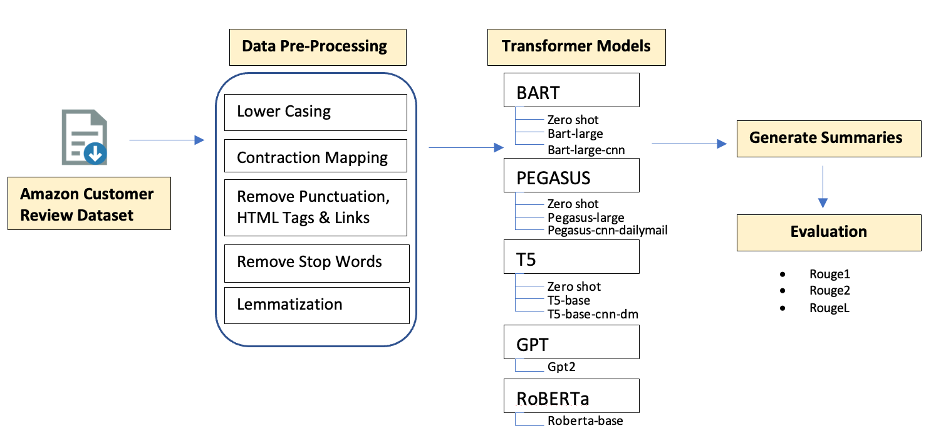
\includegraphics[width=14cm, height=7cm]{workflow.png}
\label{Fig 1. Summarization process workflow}
\end{figure}

\subsection{Dataset}
To evaluate the different transformer architectures we use the Amazon customer reviews dataset \cite{amazonDataset1, amazonDataset2} which contains user-generated reviews and summaries for a variety of products such as Home and Kitchen, Beauty, Electronics, Movies and TV etc. We filter the 200K records to extract reviews with length 0f 3000 characters or more. Furthermore we clean the extracted 11K reviews to train the transformer models on the pre-processed data. Data preprocessing is explained in detail in the Appendix. 

\subsection{Models}
For this work, we studied the following 5 popular Transformer-based models that have performed well on summarization of news articles:
\begin{enumerate}
\item {\textbf{BART} \cite{bart}: A seq2seq model with a BERT-like encoder and an autoregressive (GPT-like) decoder.}
\item {\textbf{T5}\cite{t5abstractive}: A model that uses a text-to-text approach to support multiple language understanding tasks. To perform summarization, a prefix of “summarize:” is added to each example.}
\item {\textbf{PEGASUS} \cite{pegasus}: A large model pre-trained on massive corpora with a self-supervised objective that closely resembles the summarization task leading to faster and better fine-tuning}
\item {\textbf{GPT-2}\cite{gpt2ForSummarization} : An autoregressive decoder-only model that can perform several tasks. In the original paper, to induce summarization, a “TL;DR” token was added in between the text and the summary}
\item {\textbf{RoBERTa}\cite{originalRoBerta} : RoBERTa which is an improvisation of the BERT model with modified hyperparameters, trained for larger mini batches and learning rates.}
\end{enumerate}
To better understand the performance of news summarization models on long-form user reviews, we experimented with different configurations based on the model architectures. For BART, T5, and PEGASUS, we compared three setups - a model that was not fine-tuned on our dataset (zero-shot learning), a base model fine-tuned on our dataset, and a news summarization model fine-tuned on our dataset. For both GPT-2 and RoBERTa, we did not find any existing models fine-tuned for news summarization so we were unable to do the same comparison. For these two models, we therefore focused on the performance of the base model fine-tuned on our dataset.

\subsection{Implementation}
For our compute needs, we used Google Colab Pro  \cite{GoogleColab} which gave us access to T4/P100 GPUs. We used the Huggingface Python library \cite{HuggingFace} to load pre-trained transformer models. The exact models we used are specified in Section 5. 

For fine-tuning BART, T5, and PEGASUS, we loaded the respective pre-trained models from Huggingface. For the zero-shot configuration, we used its Pipeline API \cite{Pipeline} that makes model inference easier. For the other two configurations, we used the Tokenizer object of each model to first convert text into the required format and then used the Trainer object to perform fine-tuning. To ensure consistency, we trained each model for 3 epochs, truncated input texts to 512 tokens, and used 2 beams for the beam search decoding.  Other hyperparameters such as learning rate and batch size were varied for each model based on their compute requirements and time taken. 

Similarly for RoBERTa we used the tokenizer object, RobertaTokenizerFast. Furthermore, to initialize our Seq2seq model we used the EncoderDecoderModel with roberta-base serving as both the encoder and the decoder.

For GPT-2, we were inspired by text summarization blog posts \cite{gptblog} and converted our summarization task into one of text generation to generate summaries. We concatenated the reviews in our dataset with a separator token, then appended the review title (which served as our summary). An example of what this data looked like after this processing:
\begin{center}
<|endoftext|> review body here <|body|> summary here <|EOS|>
\end{center}
Such examples were fed into the model for fine-tuning so that the model knows that the task is to generate summaries. During inference, reviews were first truncated to 200 tokens for reducing computation time and then fed into the model after adding the separator token. The decoding procedure was similar to the previous models.

\section{Results}
Similar to previous works in abstractive summarization \cite{kassasSurvey,newsSummarization, t5abstractive} , we used Recall-Oriented Understudy for Gisting Evaluation (ROUGE) scores as our evaluation metric. We used Huggingface’s ROUGE implementation to calculate the mid-range F1 scores for ROUGE-1, ROUGE-2, and ROUGE-L. ROUGE-1 and ROUGE-2 scores count the overlapping of unigrams and bi-grams respectively between the generated summaries and ground truth. ROUGE-L counts the longest common subsequence between the generated summaries and the ground truth.



\begin{table}
\caption{ROUGE scores for different transformer models }
\renewcommand{\arraystretch}{1.5}
	\centering
	\begin{tabular}{p{0.12\linewidth} | p{0.25\linewidth} | p{0.15\linewidth} |p{0.15\linewidth}|p{0.15\linewidth}}
		\hline
		\multicolumn{2}{c|}{\textbf{Pre-trained Models}} & \textbf{Rouge1} & \textbf{Rouge2} & \textbf{RougeL} \\
		\hline
		\multirow{3}{4em}{BART} & Zero Shot & 13.7 & 4.1 & 12.2 \\
        & Bart Large  & 20.1 & 8.4 & 17.9 \\
        & Bart Large CNN  & 23.0 & 10.3 & 20.7 \\ 
		\hline
		\multirow{3}{4em}{PEGASUS} & Zero Shot & 14.89 & 5.40 & 12.62\\
        & Pegasus Large  & 20.82 & 9.05 & 18.71  \\
        & Pegasus CNN Dailymail & 19.83 & 8.75 & 17.69\\ 
		\hline
		\multirow{3}{4em}{T5} & Zero Shot & 7.6 & 2.2 & 6.8\\
        & T5-base  & 17.1 & 6.5 &  15.3 \\
        & T5-base-cnn-dm & 18.7 & 8.3 & 16.4\\ 
		\hline
		\multirow{1}{4em}{GPT} & Gpt2 & 9.2 & 0.9 & 8.3\\
		\hline
		\multirow{1}{4em}{RoBERTa} & Roberta-base & 0.09 & 0 & 0.08 \\
		\hline
	\end{tabular}
\end{table}
\begin{table}[H]
\caption{Sample of generated summary for top performing models}
\renewcommand{\arraystretch}{1.5}
	\centering
	\begin{tabular}{p{0.2\linewidth} | p{0.7\linewidth} }
		\hline
		\multirow{2}{4em}{\textbf{Review}} & link video lot detail camera https //youtu.be/3c595v0a0os want watch read follow video audio camera fantastic data overlay pretty badly time sure garmin fix issue time garmin virb elite like lot audio terrible camera big improvement new xe come decide give garmin another try things want action camera 1. good video 1080p/60fps 2. good audio 3. waterproof without case sort case affects audio ...good video good audio low speed absolutely thrill camera give 5 star anticipation fix data overlay issue mention\\ 
		\hline
		\multirow{1}{4em}{\textbf{Target}} & great video audio data overlay way moment sure garmin fix 'em\\
		\hline
		\hline
		\multirow{1}{4em}{\textbf{BART} } 
         & good video good audio lot potential data overlay issue still exist need fix\\
        \hline
		\multirow{1}{4em}{\textbf{PEGASUS}}  & good video audio low speed absolutely thrill camera give 5 star \\
		\hline
		\multirow{1}{4em}{\textbf{T5} } 
        & great video quality virb elite like lot audio nice camera big improvement\\
        \hline
		\multirow{1}{4em}{\textbf{GPT}}  &  excellent video quality great audio quality excellent video playback excellent sound quality good sound excellent battery life great feature camera excellent camera software update camera \\
		\hline
	\end{tabular}
\end{table}
The ROUGE scores generated during evaluation of our models can be seen in Table 1 with the generated summaries for the top performing models in Table 2. We observed that BART performed the best out of the 5 models, getting a high of 23\%  for ROUGE-1 when using the model that was already fine-tuned on news summarization.  We hypothesize that since BART uses the bidirectional encodings of BERT with the auto-regressive decoding of GPT, it contains the best characteristics of two models that have independently good performance in several language-related tasks. We also observed that the three models that were developed with summarization in mind, namely BART, T5, and PEGASUS, performed better than the two general-purpose language models, GPT-2 and RoBERTa. PEGASUS for example was constructed specifically with downstream fine-tuning for summarization as a use-case.

Another observation is that using models that were fine-tuned on news summarization did help in performance when compared to the base models. For example our T5 experiments found an average absolute increase of 1.5 in the ROUGE score between the two configurations. We believe that this improvement can be attributed to these models’ ability to condense information and their ability to transfer this knowledge into the new domain of customer reviews.

Among all the models, RoBERTa has the worst performance. We expected it to perform fairly, but RoBERTa is known to have poor performance as it uses a Byte-Level BPE tokenizer which has poor morphological alignment with the original text. Additionally, it is not trained on text generation therefore its performance is even lower than general-purpose language models such as GPT-2 for summarization.


\section{Conclusion and Future Work}
Our experiments supported our initial hypothesis that a model’s knowledge of summarizing news articles can be successfully applied to summarizing long-form customer reviews. Our best model was a BART model fine-tuned on the CNN/Daily Mail dataset and further finetuned on our dataset which got a ROUGE-1 score of 23%.

In the future, our approach can be improved in the following ways: (1) by training on more user reviews, potentially from sources other than Amazon, (2) by calculating evaluation metrics on a larger test set. Our current approach was limited to 200 test examples due to insufficient compute. Doing the above could improve the model performance and our understanding of them.
\medskip


\bibliographystyle{abbrvnat}
\bibliography{sources}
\newpage
\begin{appendices}
\section{Team Member Contributions}
A brief summary of team contributions is as follows:

\begin{table}[H]
\caption{Summary of contributions of team member's}
\renewcommand{\arraystretch}{1.5}
	\centering
	\begin{tabular}{|p{0.1\linewidth} | p{0.8\linewidth}|}
		\hline
		{\textbf{Name }} & \textbf{Contribution} \\
		\hline
		\multirow{3}{4em}{Aditya} & Proposal Writing;\\
        & Transformer Models - T5 ( zero-shot,  t5-base, t5-base-cnn-dm) ; GPT( gpt2) : Training, Hyperparameter tuning, Generating Summaries \& Model Evaluation; \\
        & Project Report Writing  \\ 
		\hline
		\multirow{3}{4em}{Parul} & Proposal Writing;  \\
        & Data Extraction \& Pre-Processing; \\
        & Transformer Models - BART (zero-shot, bart-large, bart-large-cnn) ; RoBERTa (roberta-base) : Training, Hyperparameter tuning, Generating Summaries \& Model Evaluation ;  \\
        & Project Report Writing \\ 
		\hline
		\multirow{3}{4em}{Subhayan} & Proposal Writing; \\
        & Transformer Models - PEGASUS ( zero-shot, pegasus-large, pegasus-cnn-dailymail); GPT( gpt2) : Training, Hyperparameter tuning, Generating Summaries \& Model Evaluation; \\
        & Project Report Writing \\ 
		\hline
	\end{tabular}
\end{table}

\section{Data Preparation}
We pre-process the reviews in order to remove unwanted text and making them consistent by performing the following:
\begin{enumerate}
\item {\textbf{Lower Casing} : Convert all words to same case.}
\item {\textbf{Contraction Mapping}: Written and spoken English generally has shortened versions of words or syllables. We map the most frequently used short version to original words, for eg. i’ll → i will. }
\item {\textbf{Remove Punctuation's, HTML Tags , Links} : Removing parts of the reviews which do not add meaning to the text.}
\item {\textbf{Remove Stop Words}:Removing commonly occurring words like ‘the’, ‘a’ etc.}
\item {\textbf{Lemmatization} : It aims to remove the inflectional endings and return the base or dictionary word.}
\end{enumerate}

\section{Models}
\textbf{BART}

Bart \cite{bart} is a  seq2seq model with a BERT-like encoder and an autoregressive (GPT-like) decoder. BART pre training involves randomly shuffling the order of the original sentences. Furthermore, spans of text are replaced with a single mask token. Since, BART is trained by corrupting text with an arbitrary noising function, and learning a model to reconstruct the original text, therefore it performs well on multiple tasks like summarization, question-answering etc.In this study we finetune bart-large and bart-large-cnn model where bart-large-cnn is already fine tuned on the CNN Daily Mail and popularly used for summarisation of news articles.

\textbf{PEGASUS}

Pegasus \cite{pegasus} is an abstractive text-summarization model which involves pre-training large transformer-based encoder-decoders on massive corpora with a self-supervised objective called Gap Sentences Generation (GSG). GSG is based on the hypothesis that the use of a pre-training objective that closely resembles downstream tasks (i.e., summarization) leads to faster and better fine-tuning.  This involves important sentences being masked from  the input document are then chosen based on the Rouge1F1 scores. Pegasus was pre-trained on large corpora like C4 and HugeNews and was evaluated on 12 downstream summarization tasks spanning different domains. This model’s greatest merit is being able to perform well in low-resource summarization tasks having only a smaller amount of data to work with. Pegasus-large which was used in this work consists of 16 transformer blocks and attention heads respectively. Sinusoidal positional encoding was used in this model. For optimization, Adafactor with square root learning decay was incorporated. Finally, for decoding beam search with length penalty was used. Additionally, in this would we also fine-tuned Pegasus-CNN-Dailymail model which was finetuned on the CNN/Dailymail dataset containing news articles supplemented with bullet point summaries.

\textbf{T5}

T5 \cite{t5abstractive} is a transformer-based architecture model that uses a text-to-text approach to support multiple language understanding tasks like translation, question answering, summarization and classification. This approach enabled the use of the same loss functions and hyperparameters for various tasks. T5 has a similar architecture to BERT with the encoder and decoder consisting of 12 blocks. For optimization AdaFactor was used whereas at testing greedy decoding was incorporated. Since T5 can support multiple tasks, a task-specific text is added as prefix to the original input sequence. For pre-training purposes, T5 made use of common crawl web extracted text on which heuristic filtering was applied. T5 made use of the denoising objective which involves prediction of missing or corrupted tokens in the input. T5 made use of replacing corrupted tokens with a single sentinel token as its corruption strategy. In this work, we made use of the T5-base model and the fine-tuned version of T5 on the CNN/Dailymail dataset.

\textbf{GPT2}

GPT2 \cite{gpt2ForSummarization} is a general-purpose transformer-based learner that can translate text, summarizing passages, answering questions, and generating human-like text consists of 1.5 billion parameters and has been trained on text from 8 million websites. Unlike the popular encoder-decoder architecture, GPT-2 is a decoder only transformer. The smallest GPT2 version has 12 layers of transformers each consisting of 12 independent attention heads to capture linguistic properties. GPT-2 is based on auto-regression wherein a single token is produced at a time which is then added to the sequence of inputs. Unlike BERT, GPT-2 makes use of masked self-attention layers.Since GPT-2 can perform multiple tasks, to induce summarization behavior “TLDR” token must be added after the article to be summarized.
 We attempted to convert GPT's text generation workflow into a summarization task.  To do so, we concatenated our dataset reviews with the body tag followed by the actual dataset summaries. The end of the text tag was kept at the front of this concatenated string. This string was then fed to the autoregressive GPT2 model for fine-tuning.  For decoding we made use of beam search which was followed by the calculating of rouge scores.

\textbf{RoBERTa}

RoBERTa \cite{originalRoBerta} is an improvisation of the BERT model with modified hyperparameters, trained for larger mini batches and learning rates. It was pre-trained on the Masked Language Modeling objective using raw texts and didn’t involve any human labeling. It allowed the model to learn the bidirectional representation of a sentence contrary to traditional RNN’s and autoregressive models like GPT. Contrary to BERT it has a dynamic masking process during the training. It is mostly used in downstream tasks that involve decision making such as sequence classification or question answering. Since BART was known to have comparable performance to RoBERTa in other tasks, we choose to evaluate its performance on the summarisation task. We used the tokenizer object, RobertaTokenizerFast for preparing the input to the models. Furthermore, to initialize our Seq2seq model we used the EncoderDecoderModel with roberta-base serving as both the encoder and the decoder.

\section{Results}
Detailed examples of generated summaries using different transformer models is as follows:

\begin{table}[H]
\caption{Sample of generated summary for different models}
\renewcommand{\arraystretch}{1.5}
	\centering
	\begin{tabular}{|p{0.2\linewidth} | p{0.7\linewidth}|}
		\hline
		\multirow{2}{4em}{\textbf{Review}} & link video lot detail camera https //youtu.be/3c595v0a0os want watch read follow video audio camera fantastic data overlay pretty badly time sure garmin fix issue time garmin virb elite like lot audio terrible camera big improvement new xe come decide give garmin another try things want action camera 1. good video 1080p/60fps 2. good audio 3. waterproof without case sort case affects audio ...good video good audio low speed absolutely thrill camera give 5 star anticipation fix data overlay issue mention\\ 
		\hline
		\multirow{1}{4em}{\textbf{Target}} & great video audio data overlay way moment sure garmin fix 'em\\
		\hline
	\end{tabular}
\end{table}

\begin{table}[H]
\renewcommand{\arraystretch}{1.5}
	\centering
	\begin{tabular}{p{0.25\linewidth} | p{0.15\linewidth} | p{0.45\linewidth} }
		\hline
		\multicolumn{2}{c|}{\textbf{Models}} & \textbf{Generated Summary}  \\
		\hline
		\multirow{2}{4em}{\textbf{bart\_large\_cnn} } & \textbf{ZSL} & Action camera 1. good video 1080p/60fps 2. good audio 3. waterproof without case sort case  \\
        & \textbf{Fine Tuned}  & good video good audio lot potential data overlay issue still exist need fix\\
        \hline
		\multirow{1}{4em}{\textbf{bart\_large}} & \textbf{Fine Tuned}  & good video good audio lot potential data overlay issue still exist need fix \\
		\hline
	    \multirow{2}{4em}{\textbf{pegasus\_cnn\_dailymail} } & \textbf{ZSL} &  garmin virb elite like lot audio terrible camera big improvement new xe come decide give garmin another try things \\
        & \textbf{Fine Tuned}  & garmin virb elite action camera 1080p 60 fps great video audio low speed data overlay\\
        \hline
		\multirow{1}{4em}{\textbf{pegasus\_large}} & \textbf{Fine Tuned}  & good video audio low speed absolutely thrill camera give 5 star \\
		\hline
		\multirow{2}{4em}{\textbf{t5\_base\_cnn\_dm} } & \textbf{ZSL} & virb elite like lot audio terrible camera big improvement new xe come come decide give garmin another nice things  \\
        & \textbf{Fine Tuned}  & great video quality virb elite like lot audio nice camera big improvement\\
        \hline
		\multirow{1}{4em}{\textbf{t5\_base}} & \textbf{Fine Tuned}  & good video good audio low speed absolutely thrill camera give 5 star anticipation fix issue \\
		\multirow{1}{4em}{\textbf{gpt2}} & \textbf{Fine Tuned}  &  excellent video quality great audio quality excellent video playback excellent sound quality good sound excellent battery life great feature camera excellent camera software update camera \\
		\hline
	\end{tabular}
\end{table}






\end{appendices}

\end{document}
